\documentclass[11pt, a4paper]{article}
% ================================
%        Pakete
% ================================

\usepackage[dvips, bottom=2.5cm, top=2.5cm, right=2.5cm, left=3cm]{geometry}
\usepackage[utf8]{inputenc}
\usepackage[ngerman]{babel}
\usepackage[babel,german=quotes]{csquotes}
\usepackage[T1]{fontenc}
\usepackage{enumerate}
\usepackage{setspace}
\usepackage{mdframed}
\setstretch{1.3} 
\setlength\parindent{0pt}
\usepackage{textcomp}
\usepackage{enumerate}
\usepackage{color}
\usepackage{graphicx}
\usepackage{colortbl}
\usepackage{hhline}
\usepackage{tabularx}
\usepackage{booktabs}
\usepackage[font={footnotesize}, labelfont=bf]{caption}
\usepackage[dvipsnames]{xcolor}
\usepackage{float}
\usepackage{subfig}
%\usepackage{hhline}
\usepackage{listings}

\renewcommand{\lstlistingname}{Quelltext} 

\definecolor{deepblue}{rgb}{0,0,0.5}
\definecolor{deepred}{rgb}{0.6,0,0}
\definecolor{deepgreen}{rgb}{0,0.5,0}



% ================================
%        Quelltexte JAVA
% ================================

% Java style for highlighting
\newcommand\javastyle{\lstset{
language=Java,
basicstyle=\ttfamily\scriptsize\mdseries,
otherkeywords={self},          
keywordstyle=\ttfamily\scriptsize\mdseries\color{deepblue},
emph={MyClass,__init__},          
emphstyle=\ttfamily\scriptsize\mdseries\color{deepred},   
stringstyle=\ttfamily\scriptsize\mdseries\color{deepgreen},
commentstyle=\ttfamily\scriptsize\mdseries\color{orange},
frame=,                         
showstringspaces=false,
showtabs=true, 
tabsize=3, 
tab=,
showstringspaces=false,
numbers=left,
extendedchars=true,
breaklines=true,
numberstyle=\tiny,
numbersep=9pt,
stepnumber=1,
captionpos=b,
backgroundcolor=\color[gray]{0.95},
}}

\newcommand\javastyleoneline{\lstset{
language=Java,
basicstyle=\ttfamily\scriptsize\mdseries,
otherkeywords={self},          
keywordstyle=\ttfamily\scriptsize\mdseries\color{deepblue},
emph={MyClass,__init__},          
emphstyle=\ttfamily\scriptsize\mdseries\color{deepred},   
stringstyle=\ttfamily\scriptsize\mdseries\color{deepgreen},
commentstyle=\ttfamily\scriptsize\mdseries\color{orange},
frame=,                         
showstringspaces=false,
showtabs=true, 
tabsize=3, 
tab=,
showstringspaces=false,
numbers=left,
extendedchars=true,
breaklines=true,
numberstyle=\tiny,
numbersep=9pt,
stepnumber=1,
captionpos=b,
backgroundcolor=\color[gray]{0.95},
belowcaptionskip=0em,
belowskip=0em,
}}

% Java for external files
\newcommand\javaexternal[2][]{{
\javastyle
\lstinputlisting[#1]{#2}}}

% Java for inline
\newcommand\javainline[1]{{\javastyle\lstinline!#1!}}



% ================================
%        Quelltexte Bash
% ================================

% Bash style for highlighting (ken Abstand unter der eingefügten Bash-Zeile)
\newcommand\bashstyleoneline{\lstset{
language=BASH,
basicstyle=\ttfamily\scriptsize\mdseries,
otherkeywords={self,bash,git},          
keywordstyle=\ttfamily\scriptsize\mdseries\color{deepblue},
emph={MyClass,__init__},          
emphstyle=\ttfamily\scriptsize\mdseries\color{deepred},   
stringstyle=\ttfamily\scriptsize\mdseries\color{deepgreen},
commentstyle=\ttfamily\scriptsize\mdseries\color{orange},
frame=,                         
showstringspaces=false,
showtabs=true, 
tabsize=3, 
tab=,
showstringspaces=false,
numbers=left,
extendedchars=true,
breaklines=true,
numberstyle=\tiny,
numbersep=9pt,
stepnumber=1,
captionpos=b,
backgroundcolor=\color[gray]{0.95},
belowcaptionskip=0em,
belowskip=0em,
}}

% normaler Bash Style
\newcommand\bashstyle{\lstset{
language=BASH,
basicstyle=\ttfamily\scriptsize\mdseries,
otherkeywords={self,bash,git},          
keywordstyle=\ttfamily\scriptsize\mdseries\color{deepblue},
emph={MyClass,__init__},          
emphstyle=\ttfamily\scriptsize\mdseries\color{deepred},   
stringstyle=\ttfamily\scriptsize\mdseries\color{deepgreen},
commentstyle=\ttfamily\scriptsize\mdseries\color{orange},
frame=,                         
showstringspaces=false,
showtabs=true, 
tabsize=3, 
tab=,
showstringspaces=false,
numbers=left,
extendedchars=true,
breaklines=true,
numberstyle=\tiny,
numbersep=9pt,
stepnumber=1,
captionpos=b,
backgroundcolor=\color[gray]{0.95},
}}

% Bash Style in schwarz
\newcommand\bashstyleblack{\lstset{
language=BASH,
basicstyle=\ttfamily\scriptsize\mdseries,
otherkeywords={self,bash,git},          
keywordstyle=\ttfamily\scriptsize\mdseries\color{black},
emph={MyClass,__init__},          
emphstyle=\ttfamily\scriptsize\mdseries\color{black},   
stringstyle=\ttfamily\scriptsize\mdseries\color{black},
commentstyle=\ttfamily\scriptsize\mdseries\color{black},
frame=,                         
showstringspaces=false,
showtabs=true, 
tabsize=3, 
tab=,
showstringspaces=false,
numbers=left,
extendedchars=true,
breaklines=true,
numberstyle=\tiny,
numbersep=9pt,
stepnumber=1,
captionpos=b,
backgroundcolor=\color[gray]{0.95}
}}

% BASH for external files
\newcommand\bashexternal[2][]{{
\bashstyle
\lstinputlisting[#1]{#2}}}

% BASH for inline
\newcommand\bashinline[1]{{\bashstyle\lstinline!#1!}}



\begin{document}
%\pagestyle{empty}
\section*{Anschluss von Bauteilen an den Raspberry Pi}

Am Raspberry Pi können verschiedene Bauteile angeschlossen werden, welche die Objekte repräsentieren sollen. Dazu verfügt jedes Bauteil über Anschlüsse, die auf dem Steckbrett mit dem GPIO des Raspberry Pi verbunden werden müssen. Dabei ist es wichtig, die Kabel so zu stecken, wie es die Anschlüsse auf dem Bauteil vorschreiben.\\

In Tabelle \ref{table:pinb_legung_bcm} ist noch einmal der GPIO abgedruckt. Die Pinne, die mit ">IO"< beginnen, werden genutzt, um die Bauteile zu steuern oder den Zustand der Bauteile auszulesen. In Abbildung \ref{fig:bauteile_steckbrett} werden zwei Beispiele gegeben, wie die Bauteile anzuschließen sind. Benötigt ein Bauteil einen Anschluss für ">+3,3V"< oder ">GND"<, kann ein beliebiger ">3V3"<- oder ">GND"<-Pin ausgewählt werden.

% Alternativ zu den Bildern (folgen): 
% Abstrakte Tabelle zum Anschluss eines Lichtsensors (Phototransistor)
%\begin{table}[htbp]
%  \centering
%  \begin{tabular}{@{} ccc @{}}
%    \toprule
%    Lichtsensor &  & GPIO \\ 
%    \midrule
%    PIN & $\qquad\longleftrightarrow\qquad$ & IO11 \\ 
%    \textcolor{red}{+3,3V} & $\longleftrightarrow$ & 3V3 \\ 
%    \textcolor{blue}{GND} & $\longleftrightarrow$ & GND \\ 
%    \bottomrule
%  \end{tabular}
%  \caption{Anschluss eines Lichtsensors.}
%  \label{table:anschluss_lichtsensor}
%\end{table}

\subsection*{Anschließen und Anschalten eines Bauteils}
Zum Anschließen und Anschalten eines Bauteils geht man so vor:

\begin{enumerate}

\item Raspberry Pi ausschalten.

\item Das Bauteil mit Jumper-Kabeln mit dem GPIO des Raspberry Pi verbinden. Dazu ist auf jedem Bauteil vorgegeben, wie die Kabel gesteckt werden müssen. \textbf{Bitte noch einmal vergewissern, dass das Bauteil richtig angeschlossen wurde!}

\item Raspberry Pi einschalten (und ggfs. einloggen).

\item Groovy-Shell starten: Dazu muss das Terminal gestartet werden und in den Ordner der Installation der ">rpCollection"< navigiert werden. Dort kann dann mit dem Befehl
\lstset{language=Bash}
\bashstyle 
\begin{lstlisting}
bash start.sh
\end{lstlisting}
die Groovy-Shell aufgerufen werden. Dies kann ein paar Sekunden dauern.

\item Nun kann mit den Bauteilen gearbeitet werden: Dafür muss für jedes Bauteil ein Objekt erzeugt werden. Natürlich muss bei der Objekterstellung auch der Pin angegeben werden, an den es angeschlossen ist (also z.\,B. 11 für ">IO11"<).

Im Quelltext \ref{listing:einfache_led} ist ein Beispiel gegeben, wie die Befehle zum Schalten eines Scheinwerfers (einer LED) lauten. Zunächst wird ein Objekt für eine gelbe LED erstellt, die an Pin 11 angeschlossen ist. Dann wird diese eingeschaltet\footnote{Der Attributwert des Attributs \javainline{status} ändert sich beim Ein- bzw. Ausschalten des Lichts automatisch.} und danach der Attributwert für das Attribut \javainline{standort} geändert.
\item Es kann mit den im Unterricht modellierten Objekten gearbeitet werden: 

Scheinwerfer, RGBScheinwerfer, Helligkeitssensor und Hintergrundbeleuchtung.

\item Sollte einmal unklar sein, wie eine Methode bei einem Bauteil heißt, gibt es eine Dokumentation im Ordner ">Dokumentation"< im Installationsordner der ">rpCollection"<. Diese wird über die Datei \texttt{index.html} geöffnet. In der linken Seitenleiste können dann z.\,B. alle Informationen zum RGBScheinwerfer aufgerufen werden.  

\end{enumerate}

\lstset{language=Java}
\javastyle 
\begin{lstlisting}[caption={Steuerung eines Scheinwerfers.},label={listing:einfache_led}]
// Dies ist ein Kommentar. Er wird nicht weiter beachtet.

// Erzeuge das Objekt 'gelbeLampe' fuer die LED, die an Pin 11 (IO11) angeschlossen ist:
gelbeLampe = new Scheinwerfer(11);

// Nun soll eine Methode bei einem Objekt aufgerufen werden.
// Beispiel: 
// Rufe die Methode 'anschalten()' beim Objekt 'gelbeLampe' auf
gelbeLampe.anschalten()

// Der Aufruf funktioniert immer so: 
// <OBJEKTNAME>.<METHODENNAME>
// Achtung: Die runden Klammern beim Methodennamen duerfen nicht vergessen werden.
// Hat eine Methode einen Parameter, so muss der Parameterwert in den runden Klammern angegeben werden. Mehrere Parameterwerte sind durch Kommata zu trennen (auf die Reihenfolge achten!).

// Setze den Attributwert 'Martins Buehne' fuer das Attribut 'standort' fuer das Objekt 'gelbeLampe':
// Zeichenketten sind in Anfuehrungszeichen zu setzen.
gelbeLampe.setzeStandort("Martins Buehne");
\end{lstlisting}

\begin{figure*}[htb]
    \centering
    %\fbox{
     \subfloat[Anschluss des RGB-Scheinwerfers (Anschluss an ">IO02"<, ">IO03"<, ">IO04"< und ">GND"<).]{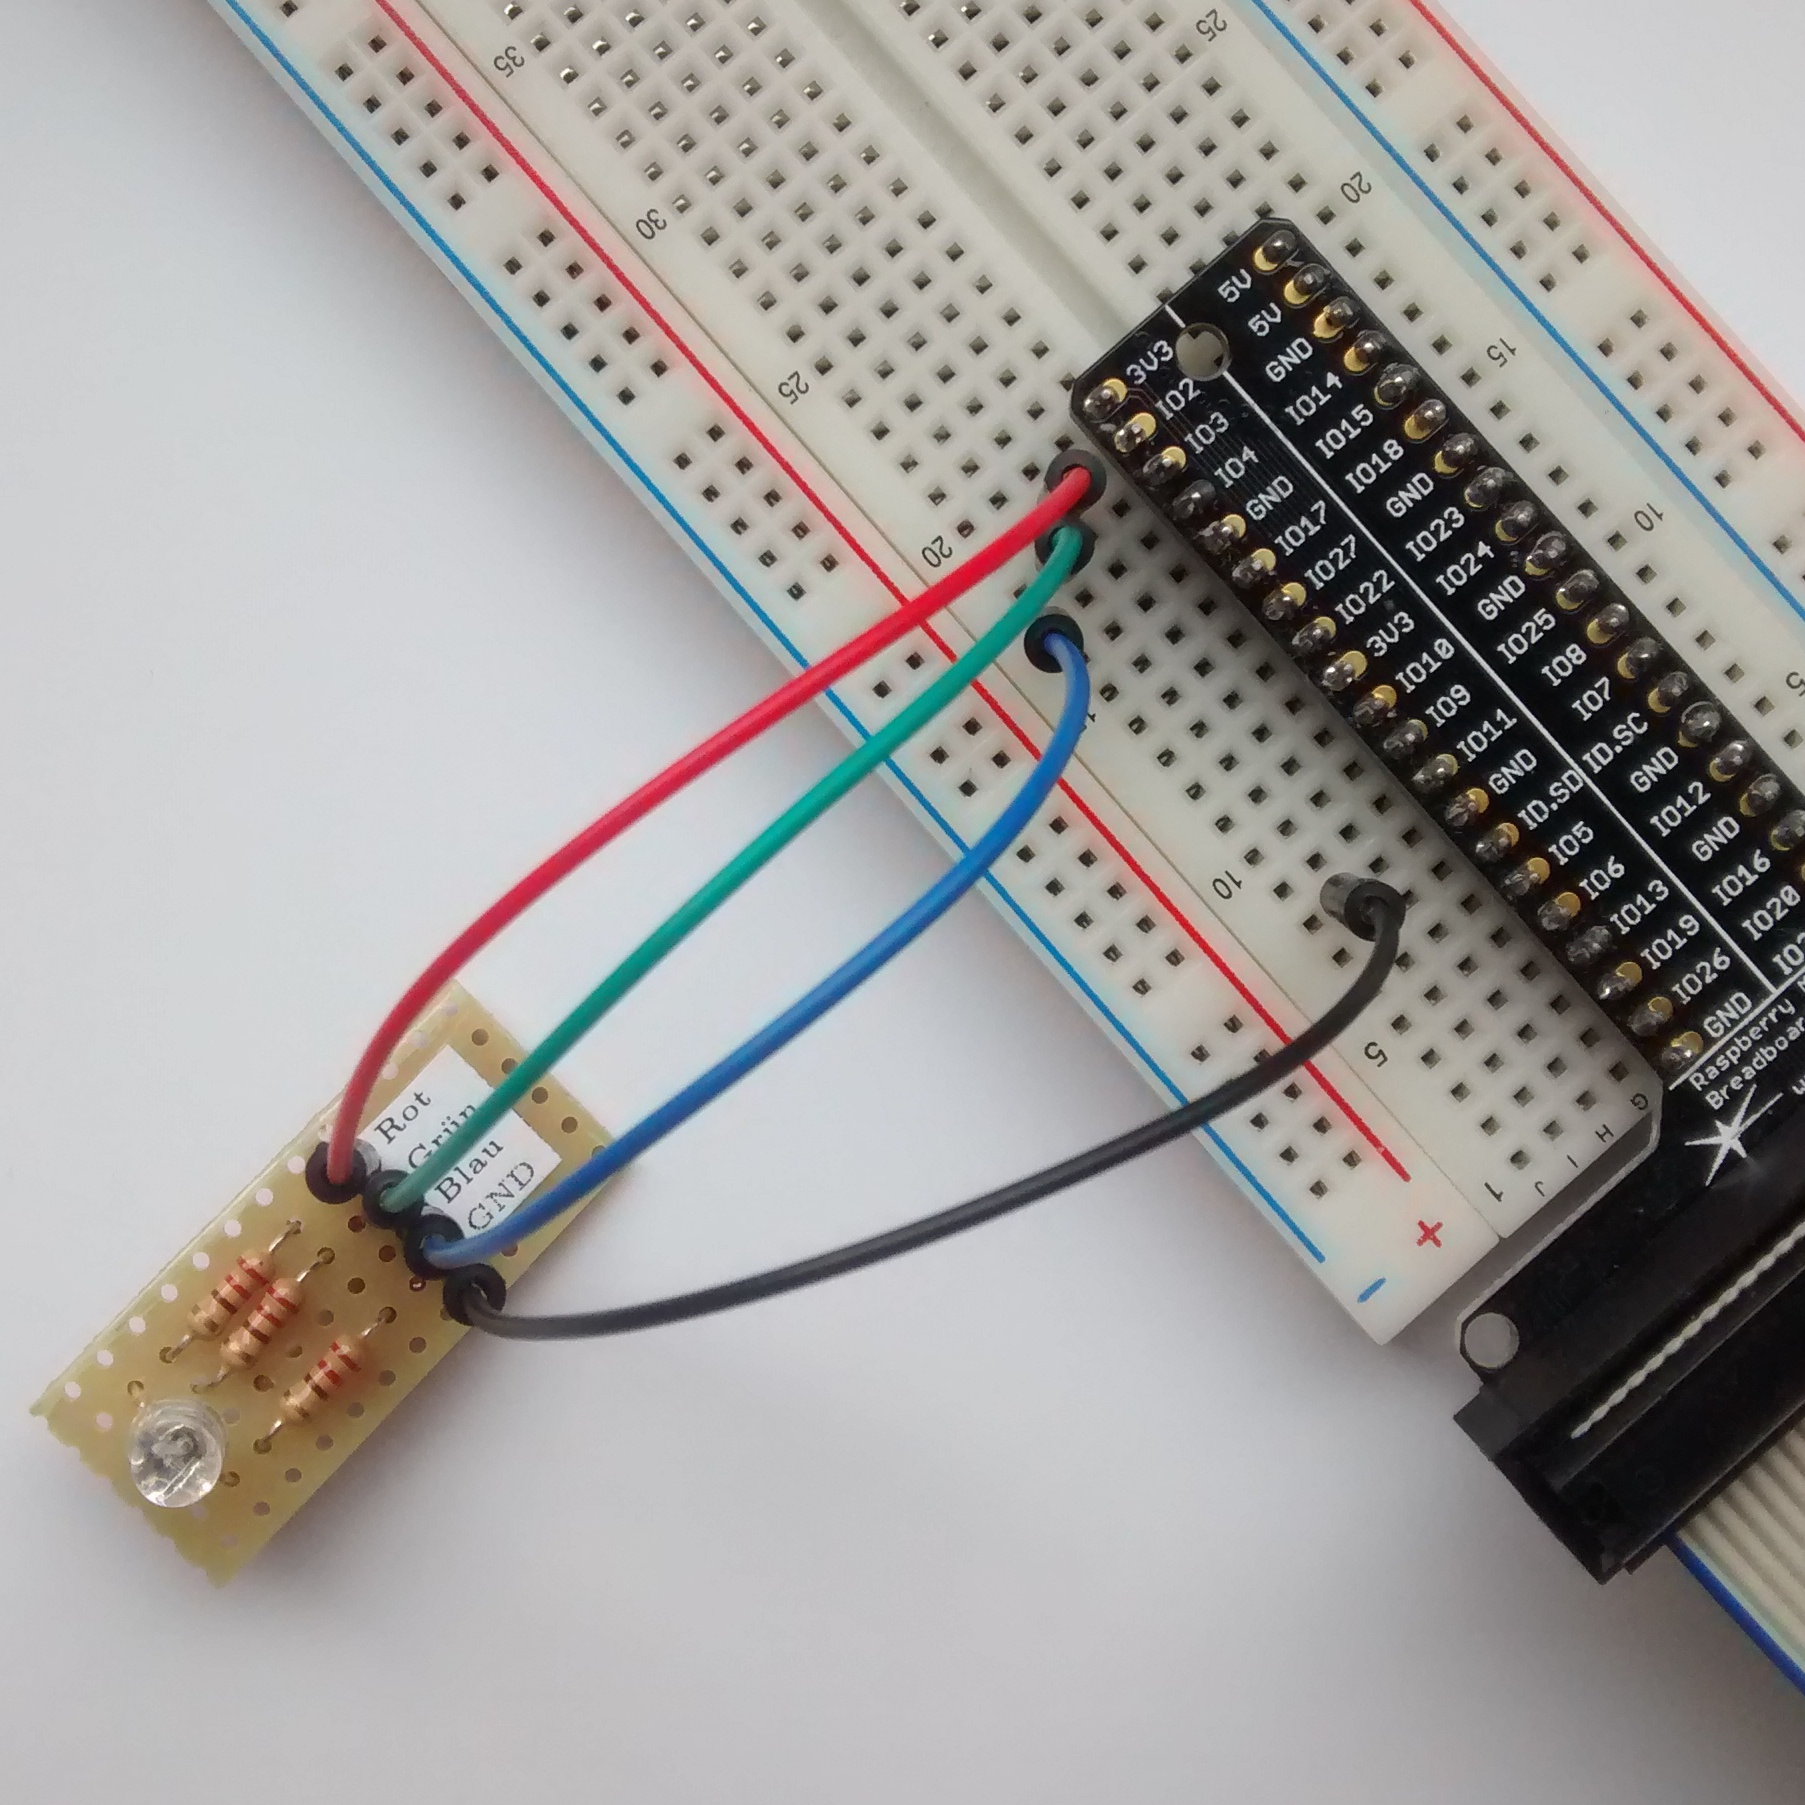
\includegraphics[width=7.5cm]{img/anschluss_rgb_led}}
     ~
       \subfloat[Anschluss eines Helligkeitssensors (Anschluss an ">IO03"<, ">3V3"< und ">GND"<).]{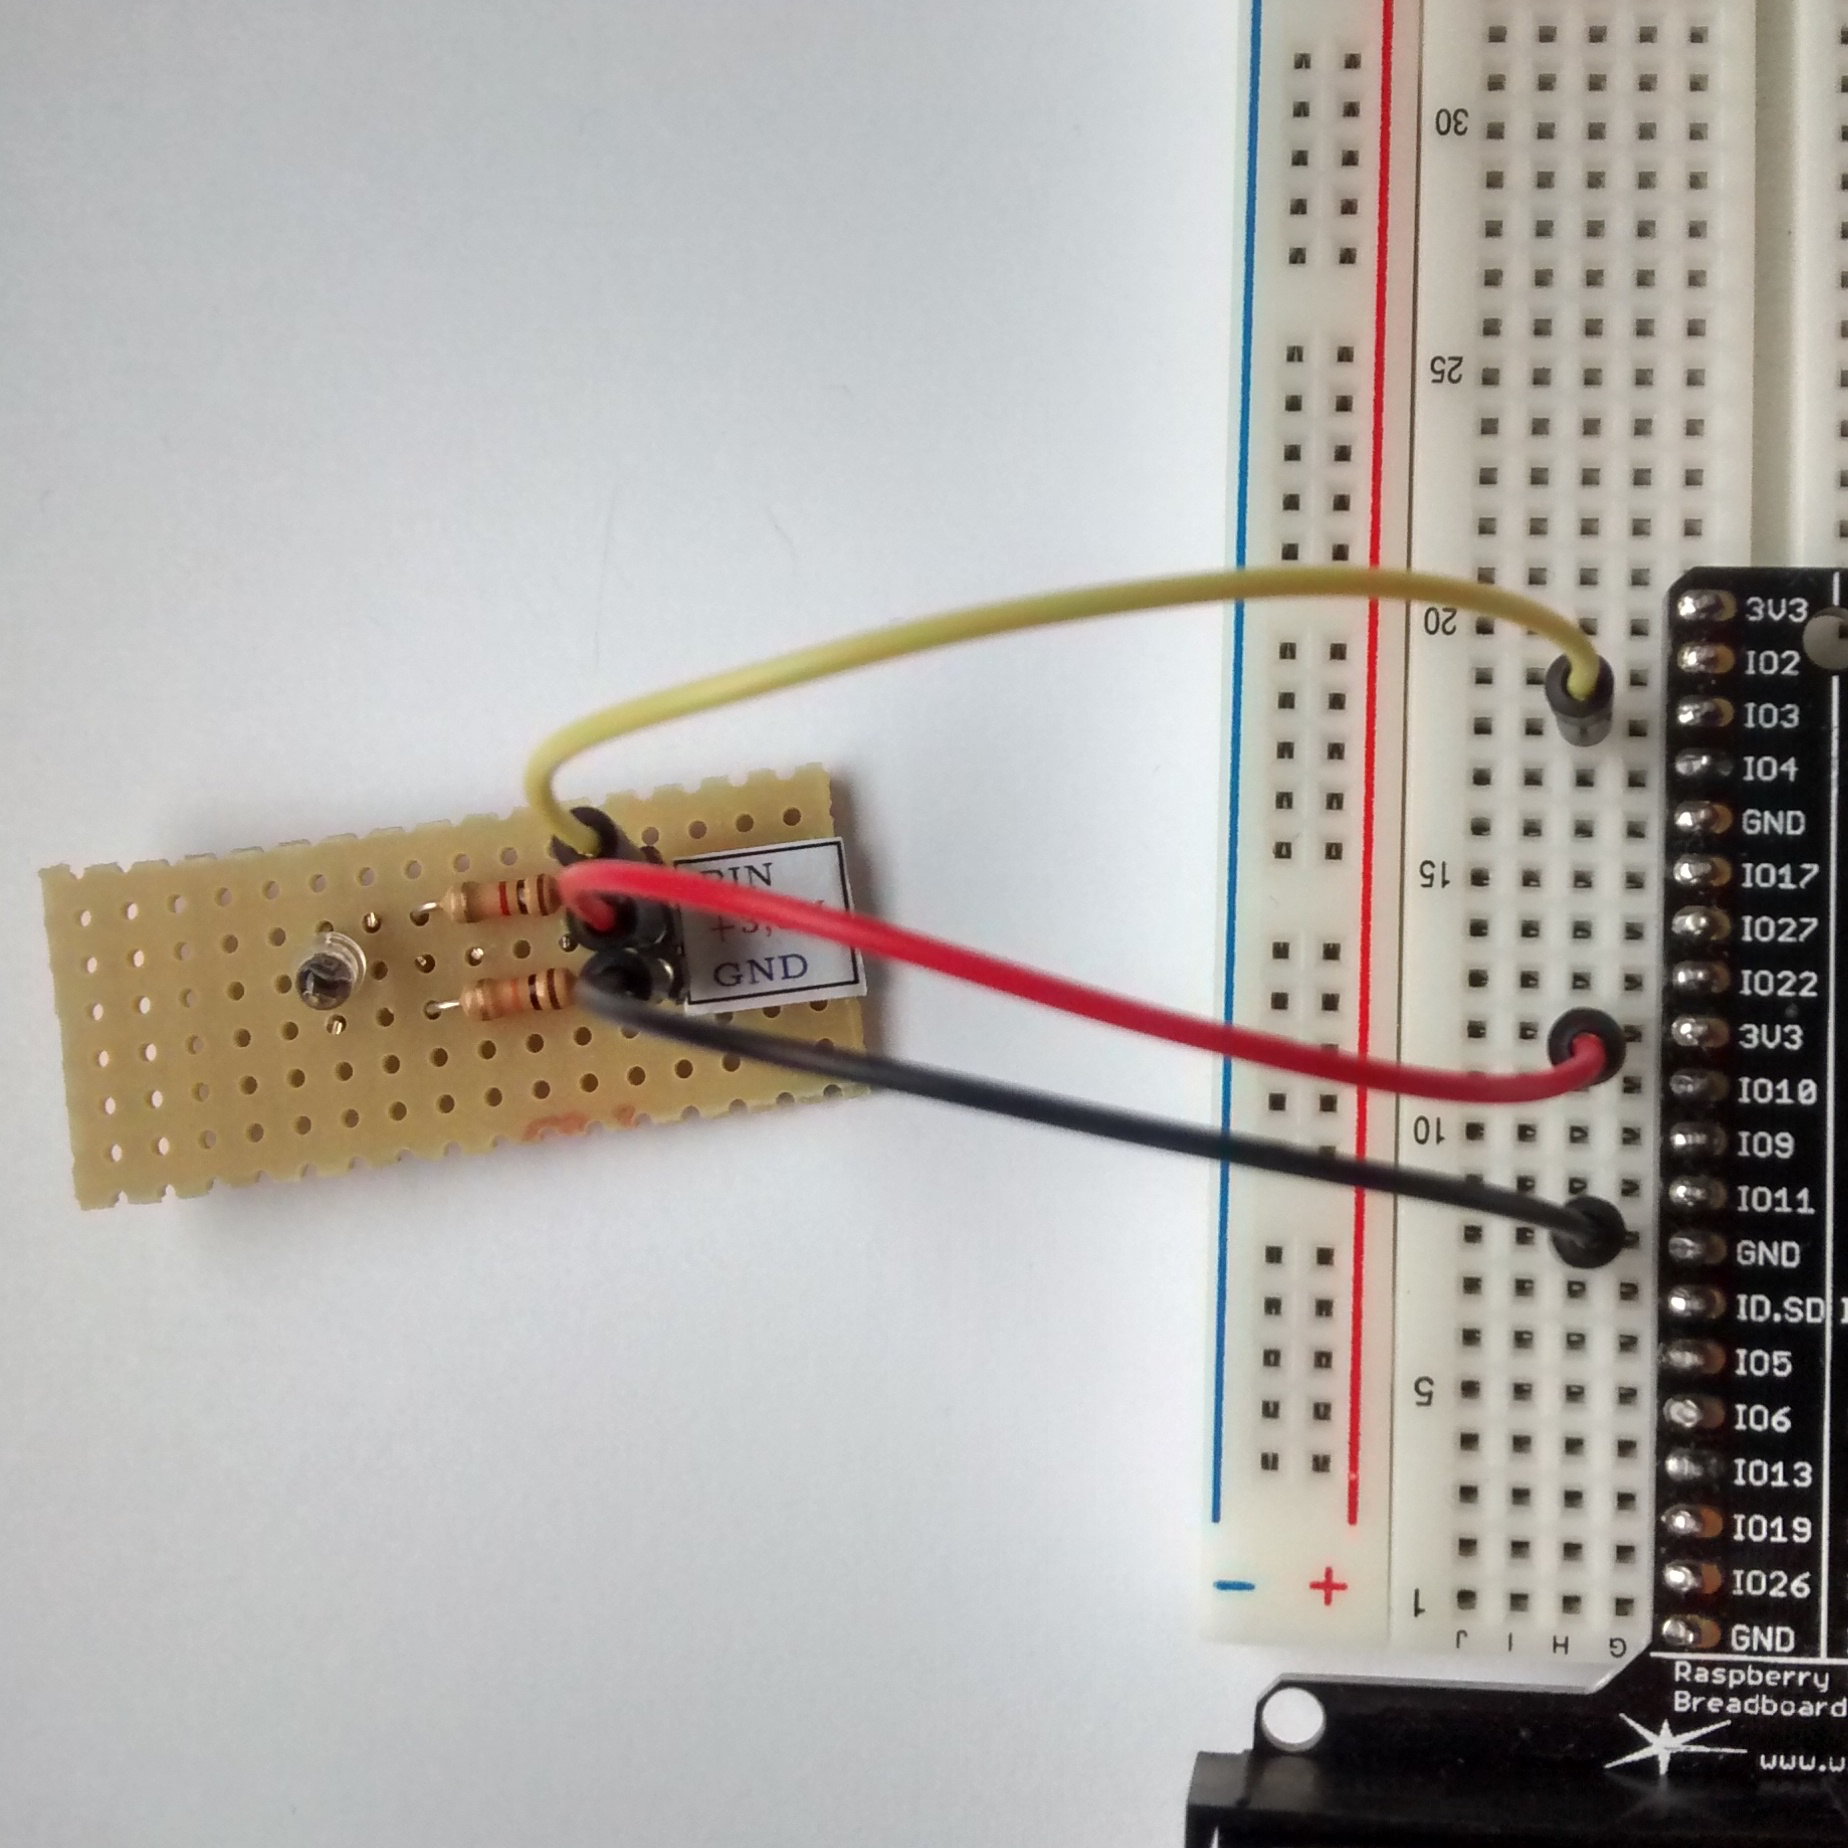
\includegraphics[width=7.5cm]{img/anschluss_phototransistor}}
    \caption{Angeschlossene Bauteile am Steckbrett.}
    \label{fig:bauteile_steckbrett}
\end{figure*}









% Folgendes evtl. in eigene Datei auslagern:
\newpage
\begin{table}[htb]
\centering
\scalebox{1}{
\begin{tabular}{>{\columncolor[gray]{1}}ll|>{\columncolor[gray]{0.9}}c >{\columncolor[gray]{0.9}}c|rr}
\multicolumn{1}{l}{} & \multicolumn{1}{l}{\textbf{BCM}} & \multicolumn{1}{c}{}  & \multicolumn{1}{c}{}  & \multicolumn{1}{r}{\textbf{BCM}} & \multicolumn{1}{r}{}   
\vspace{3mm}\\
\arrayrulecolor[gray]{0}
\hhline{>{\arrayrulecolor[gray]{1}}-->{\arrayrulecolor[gray]{0}}|--|>{\arrayrulecolor[gray]{1}}--|}
\arrayrulecolor[gray]{0}
& 3V3 & $\bullet$ & $\bullet$ & 5V &  \\
& IO2 & $\bullet$ & $\bullet$ & 5V & \\
& IO3 & $\bullet$ & $\bullet$ & GND & \\
& IO4 & $\bullet$ & $\bullet$ & IO14 &  \\
& GND & $\bullet$ & $\bullet$ & IO15 &  \\
& IO17 & $\bullet$ & $\bullet$ & IO18 &  \\
& IO27 & $\bullet$ & $\bullet$ & GND &  \\
& IO22 & $\bullet$ & $\bullet$ & IO23 &  \\
& 3V3 & $\bullet$ & $\bullet$ & IO24 &  \\
& IO10 & $\bullet$ & $\bullet$ & GND &  \\
& IO9 & $\bullet$ & $\bullet$ & IO25 &  \\
& IO11 & $\bullet$ & $\bullet$ & IO8 &  \\
& GND & $\bullet$ & $\bullet$ & IO7 &  \\
& ID.SD & $\bullet$ & $\bullet$ & ID.SC &  \\
& IO5 & $\bullet$ & $\bullet$ & GND &  \\
& IO6 & $\bullet$ & $\bullet$ & IO12 &  \\
& IO13 & $\bullet$ & $\bullet$ & GND &  \\
& IO19 & $\bullet$ & $\bullet$ & IO16 &  \\
& IO26 & $\bullet$ & $\bullet$ & IO20 & \\
& GND & $\bullet$ & $\bullet$ & IO21 & \\
\hhline{--|>{\arrayrulecolor[gray]{0.9}}-->{\arrayrulecolor{black}}|--|}
\rowcolor[gray]{0.9}
\multicolumn{1}{|c}{} & \multicolumn{1}{c}{}  & \multicolumn{1}{c}{} & \multicolumn{1}{c}{} & \multicolumn{1}{c}{} & \multicolumn{1}{c|}{} \\
\hline
\end{tabular}
}
\caption{Pin-Belegung auf dem GPIO (BCM-Layout).}
\label{table:pinb_legung_bcm}
\end{table}

\end{document}
